

\section{Particle Dynamics}
\label{sec:particledynamics}
Population balance models rely on the Eulerian description of particles where average properties of particle population such as number density, mass or surface area are treated as continuous quantities and tracked by solving scalar transport equations. These methods are computationally cheaper compared with mesoscale models such as DEM, and can be easily interfaced with chemical kinetics in CFD solvers to simulate soot formation in laminar and turbulent configurations. Here, we use two particle dynamics models: a monodisperse population balance model (MPBM), which tracks four variables and results in four transport equations, and a fixed sectional population balance model (SPBM), which tracks three variables per section. In the SPBM approach, the total number of transport equations equals the number of tracked variables multiplied by the number of sections. 

Having the total number concentration of agglomerates and primary particles and total carbon content of soot enables the model to describe evolving fractal-like morphology and surface area of soot agglomerates, which is essential to compute their collision frequency~\citep{mulholland1988cluster} as well as oxidation and surface growth rates~\citep{kelesidis2019estimating}. Tracking hydrogen content of soot allows capturing the soot composition, thereby its maturity~\citep{kholghy2016core}, and surface reactivity~\citep{blanquart2009analyzing}.

The common features of implemented particle dynamics models are reviewed in Section~\ref{sec:pdynamiccommon}. The composition (H/C), diffusion coefficient, and morphology of soot particles are calculated in the same manner for MPBM and each section in SPBM. However, particle dynamics models differ in terms of the calculation of coagulation, and the processing of the contributions from inception, surface growth, and coagulation to generate the source terms of soot variables, $S_{\varphi}$, incorporated into the transport equations.

\subsection{Common Features}
\label{sec:pdynamiccommon}
\subsubsection{Soot Morphology}
\label{sec:sootmorphology}

The evolving fractal-like structure of agglomerates is quantified by their mobility diameter normalized by primary particle diameter, $d_m/d_p$, and gyration diameter, $d_m/d_g$, that can be described with power-laws derived from mesoscale simulations.
Incipient soot is initially a sphere formed of PAHs that grows in size by surface reactions and forms agglomerates by coagulation. The collision frequency of particles depends on their evolving fractal-like structure~\citep{mulholland1988cluster}.
Mobility and gyration diameters are calculated using power-laws developed to describe the morphology of soot from premixed~\citep{abid2008evolution}, diffusion~\citep{yon2015simple} flames, and diesel engines~\citep{rissler2013effective}. Figure~\ref{fig:Morphology} shows the schematic of a soot agglomerate composed of 12 primary particles, with ${d_p}$, ${d_m}$, and ${d_g}$ annotated.
\begin{figure}[!htbp]
	\centering
	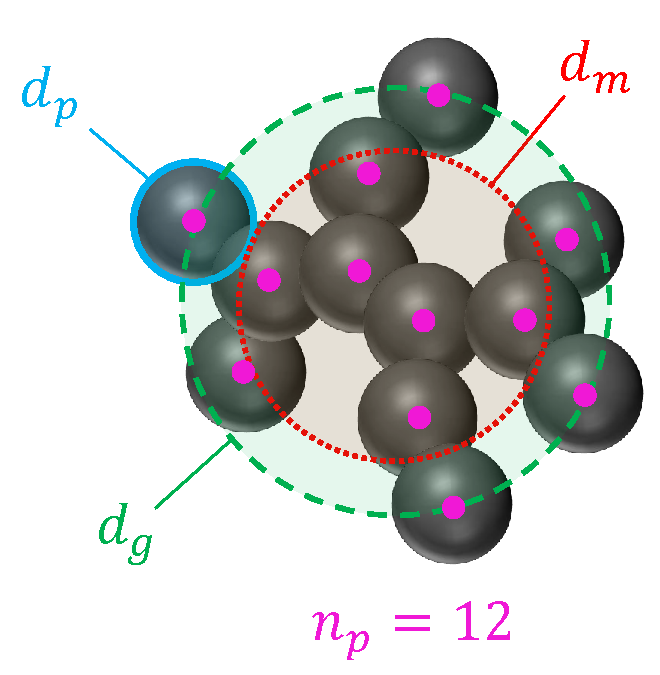
\includegraphics[height=60mm, ]{Figures/Theory/Morphology.pdf}
	\caption{The schematics of a soot agglomerates with 12 primary particles (${n_p=12}$). Primary particle, ${d_p}$, mobility ${d_m}$, and gyration ${d_g}$, diameters are shown.}
	\label{fig:Morphology}
\end{figure} 


${n^i_p}$ is the number of primary particles per agglomerate of the ${i^{th}}$ section that can be obtained by dividing the number concentration of primary particles in the ${i^{th}}$ section by that of agglomerates in that section as:


\begin{equation}
	n^i_p = \frac{N^i_{pri}}{N^i_{agg}}
	\label{eqn:n_p}.
\end{equation}

The primary particle diameter, ${d^i_p}$, is determined from the total carbon content and the number density of primary particles using:

\begin{equation}
	d^i_p = \left(\frac{6}{\pi} \frac{C^i_{tot}\cdot W_{carbon}}{\rho_{soot}} \frac{1}{N^i_{pri}\cdot Av} \right)^{1/3}.
	\label{eqn:d_p}
\end{equation}

The DEM-derived power-laws~\citep{Kelesidis2017} relate ${d^i_m}$ and ${d^i_g}$ to ${d^i_p}$ and ${n^i_p}$ as:

\begin{equation}
	d^i_{m} = d^i_p\cdot {n^i_p}^{0.45}
	\label{eqn:d_m},
\end{equation}

\begin{equation}
	d^i_g = 
	\left\{
	\begin{array}{lr}
		d^i_m/({n^i_p}^{-0.2}+0.4), & \text{if } n^i_p > 1.5\\
		d^i_m/1.29 & \text{if } n^i_p\leq 1.5
	\end{array}
	\right.
	\label{eqn:d_g}
\end{equation}

The collision diameter, ${d^i_c}$, is the maximum of ${d^i_{m}}$ and ${d^i_{g}}$:

\begin{equation}
	d^i_c = \mathrm{max}\left(d^i_m, d^i_g\right).
	\label{eqn:d_c}
\end{equation}

The volume equivalent diameter, $d^i_v$, is the diameter of the sphere with the same mass as the agglomerate, and it is obtained as:
\begin{equation}
	d^i_v = d^i_p \cdot {n^i_p}^{1/3}.
	\label{eqn:d_v}
\end{equation}

The primary particle surface area is calculated from ${d^i_p}$ assuming spherical primary particles as:
\begin{equation}
	A^i_{p} = \pi {d^i_p}^2.
	\label{eqn:Ap}
\end{equation}
$A^i_{tot}$ (for each section) is defined as the total surface area of soot particles per unit mass of gas mixture obtained as:
\begin{equation}
	A^i_{tot} = N^i_{pri}\cdot Av\cdot A^i_{p}
	\label{eqn:Atot}.
\end{equation}

Mass of each agglomerate, $m^i_{agg}$ is expressed as:
\begin{equation}
	m^i_{agg} = \frac{C^i_{tot}\cdot W_{carbon}}{N^i_{agg}\cdot Av}.
	\label{eqn:m_agg}
\end{equation}


\subsubsection{Soot Composition}
\label{sec:sootcomp}
The composition of soot characterized by their elemental carbon to hydrogen ratio (C/H) is a measure of soot maturity and increases from $\mathrm{C/H<2}$ for incipient soot~\citep{ciajolo1998spectroscopic} to $\mathrm{2<C/H<10}$ for nascent soot~\citep{betrancourt2017investigation} and $\mathrm{C/H>20}$ for mature soot~\citep{michelsen2017probing}. The soot agglomerates are assumed to have pure carbon graphitic core~\citep{kholghy2016core} with all hydrogen atoms on the surface~\citep{blanquart2009analyzing}. C/H ratio can be obtained from the total carbon and the hydrogen content as:

\begin{equation}
	\left(
	\frac{C}{H}
	\right)^i
	=\frac{C^i_{tot}}{H^i_{tot}}   
	\label{eqn:CtoH}.
\end{equation}

The carbon content of each agglomerate is a predefined parameter in the SPBM (depending on the section the agglomerate is placed), but it can be calculated from dividing ${C_{tot}}$ by ${N_{agg}}$ for the MPBM. The hydrogen content of each agglomerate is calculated for both particle dynamics models as:

\begin{equation}
	H^i_{agg}
	=\frac{H^i_{tot}}{N^i_{agg}}   
	\label{eqn:Hagg}.
\end{equation}


\subsubsection{Diffusion of soot particles}
% [Might be removed to the supplumenatary material for the paper]
The diffusion coefficient of soot particle, $D^i$, is calculated as:

\begin{equation}
	D^i = \frac{k_B T}{f^i}
	\label{eqn:diff},
\end{equation}
\noindent where $f^i$ is the friction factor of particles in the gas mixture, and it is calculated as:

\begin{equation}
	f^i = \frac{3\pi\mu d^i_m}{C^i(d^i_m)},
	\label{eqn:fraction}
\end{equation}

\noindent where ${C^i}$ is the Cunningham correction factor for the particle friction factor that accounts for non-continuum effects in the transition and free molecular regimes. ${C^i}$ is calculated for a given diameter, $d$, as: 
\begin{equation}
	C^i(d) = 1+\frac{2\lambda}{d}
	\left(
	1.21+0.4\mathrm{exp}(\frac{-0.78d}{\lambda})
	\right)
	\label{eqn:cun},
\end{equation}
\noindent  where $\lambda$ is the mean free path of gas given as:
\begin{equation}
	\lambda = \frac{\mu}{\rho}\sqrt{\frac{\pi W_{gas}}{2k_B Av T}}
	\label{eqn:lambda}.
\end{equation}
Note that $\lambda$ is a property of the gas mixture that does not depend on particle mass and morphology. 


\subsection{Sectional Population Balance Model}
A SPBM with fixed pivots is used to describe particle dynamics~\citep{wu1988discrete}. The mass range of particles is divided into discrete sections each of which includes agglomerates of the same mass. Figure~\ref{fig:sectional} illustrates the interaction between the gas phase and mass sections, as well as the mechanisms by which particles move between sections. Inception introduces new particles to the first section with the mass corresponding to the incipient particle. The particles of each section can migrate to upper sections by gaining mass via surface growth and coagulation, and return to lower sections when they lose mass through oxidation without breaking into smaller particles (i.e., fragmentation is not considered). Particles attach at point contact without coalescence. The mass of sections is determined by a geometric progression that has an initial value equal to the mass of incipient soot particle, and a common ratio of SF, known as sectional spacing factor. The mass of each section is approximated by the carbon content of agglomerates in moles as:

\begin{equation}
	C^i_{agg} = \frac{n_{c,min}}{Av}\cdot SF^{(i-1)},
	\label{eqn:Caggsec}
\end{equation}
\noindent where $(i-1)$ represents the exponent of SF. The mass of hydrogen is ignored in the placement of agglomerates in the sections.
The total number density of agglomerates, $N^i_{agg}$, and primary particles, ${N^i_{pri}}$, and the hydrogen content, $H_{tot}$, are tracked for each section. The mass of each section is fixed, so $C_{tot}$, for each section can be easily calculated by knowing the number of agglomerates; that is, $C_{tot} = N^i_{agg} \cdot {Av} \cdot C^i_{agg}$. Morphological parameters for each section are determined according to the equations provided in Section~\ref{sec:sootmorphology}.


\begin{figure}[!htbp]
	\centering
	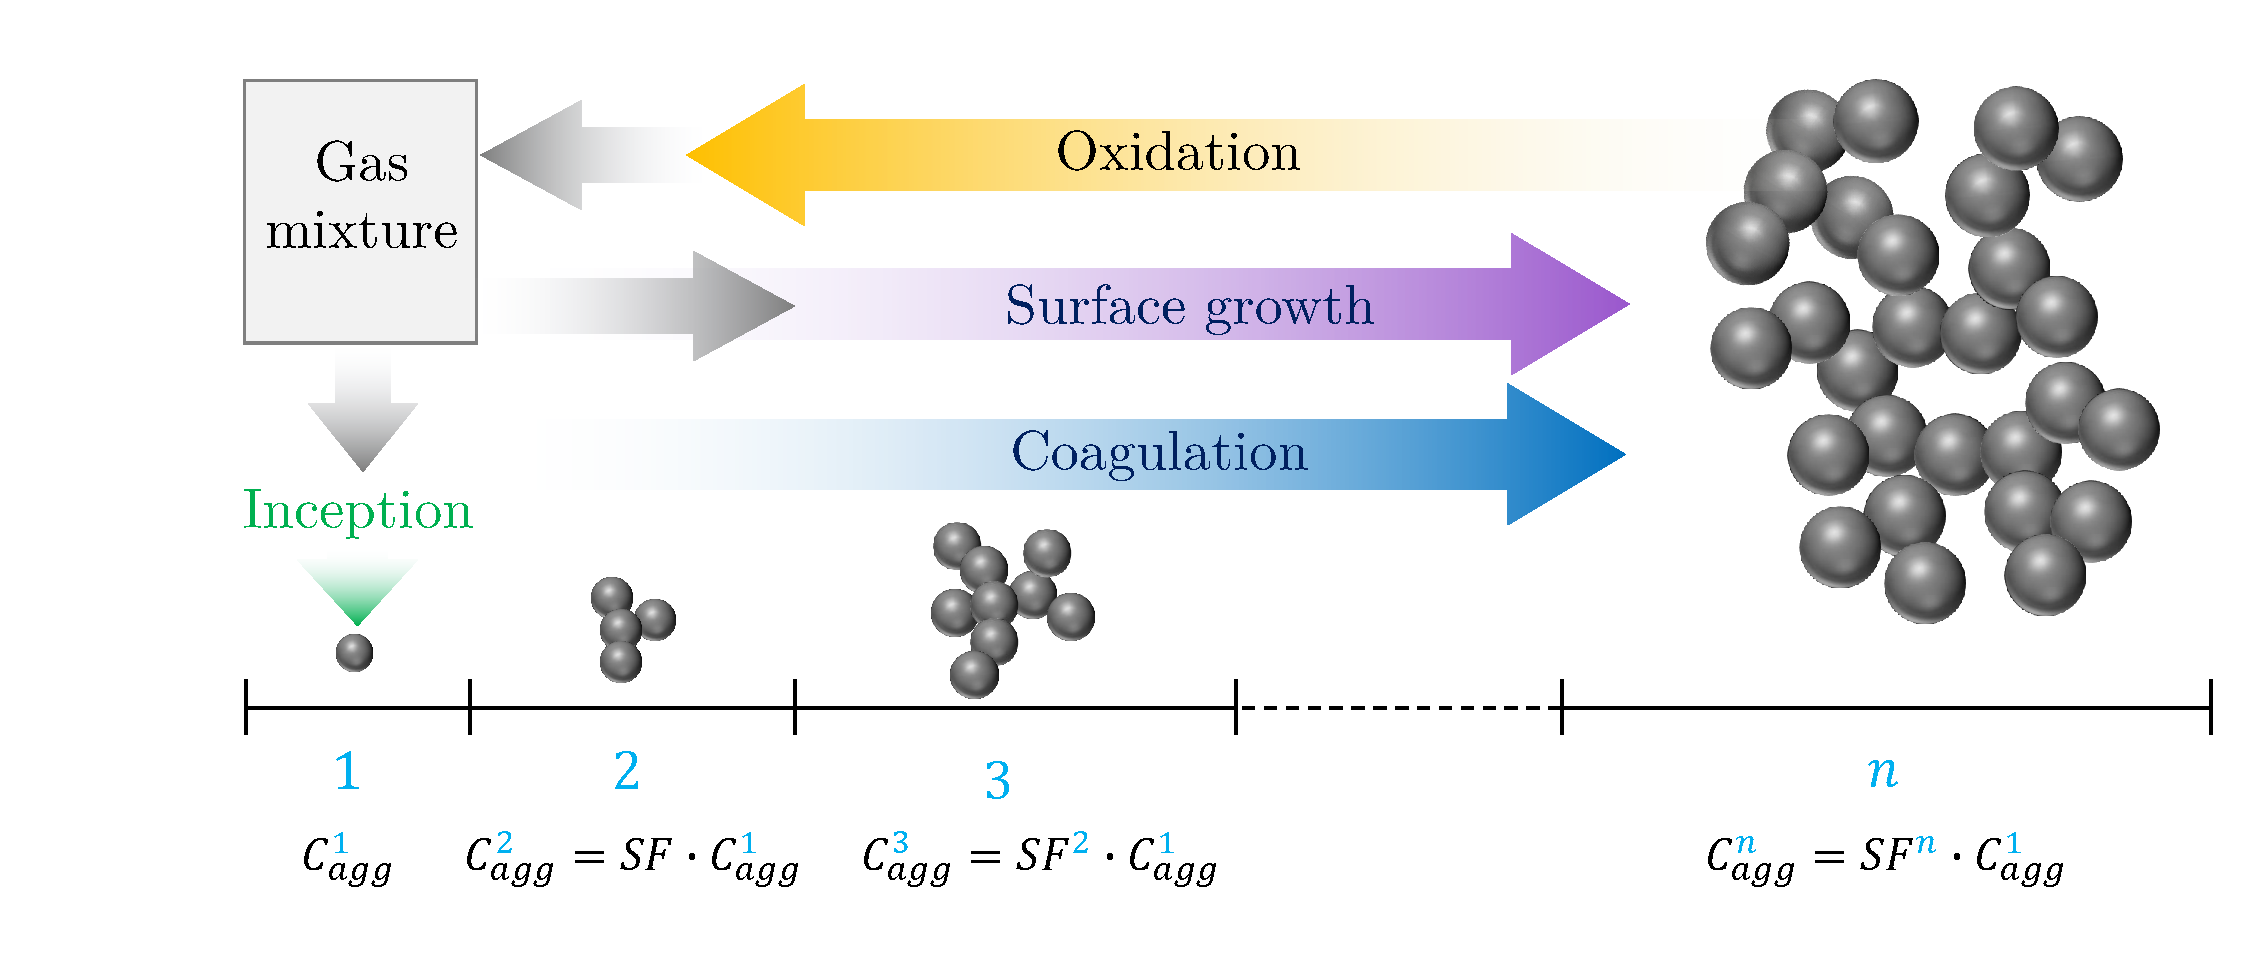
\includegraphics[height=40mm, ]{Figures/Theory/Sectional.pdf}
	\caption{The illustration of sections in SPBM. The mass of sections grows progressively by the scale factor of SF. Inception introduces new particles to the first section that propagate to the upper section via coagulation and surface growth and return to lower sections by oxidation. Carbon and hydrogen pass from gas to solid phase through inception and surface growth and goes back via oxidation.}
	\label{fig:sectional}
\end{figure}
 
New particles formed by coagulation are assigned to an upper section, with a total mass equal to the sum of the masses of the colliding particles. If the mass of resulting particle falls between two consecutive sections, the mass is distributed between them proportionally. In some cases, the mass of the newly formed particle may exceed the upper bound of the last section, causing it to fall outside the tracked mass range. This leads to potential mass loss, which is a known limitation of the fixed pivot sectional model~\citep{zhang2010detailed}. However, this issue can be mitigated by choosing an appropriate number of sections and a suitable spacing factor to ensure the uppermost sections remain unoccupied during the simulation. In the SPBM, the source terms of tracked soot variables (which appear in Equations~\ref{eqn:sootconstuv},~\ref{eqn:sootpsr},~and~\ref{eqn:sootpfr}) are split into four parts showing the contribution of inception, surface growth, oxidation and coagulation. The effect of HACA and PAH adsorption are combined (denoted by the subscript \textit{haca,ads}) because they are similar mass-gaining mechanisms. The source terms for section $i$ are given as:

\begin{equation}
	S^i_{N_{agg}} = 
	\left(S^i_{N_{agg}}\right)_{inc}
	+\left(S^i_{N_{agg}}\right)_{haca, ads}
	+\left(S^i_{N_{agg}}\right)_{ox}
	+\left(S^i_{N_{agg}}\right)_{coag}
	\label{eqn:S_Naggsect},
\end{equation}

\begin{equation}
	S^i_{N_{pri}} = 
	\left(S^i_{N_{pri}}\right)_{inc}
	+\left(S^i_{N_{pri}}\right)_{haca, ads}
	+\left(S^i_{N_{pri}}\right)_{ox}
	+\left(S^i_{N_{pri}}\right)_{coag}
	\label{eqn:S_Nprisect},
\end{equation}

\begin{equation}
	S^i_{H_{tot}} = 
	\left(S^i_{H_{tot}}\right)_{inc}
	+\left(S^i_{H_{tot}}\right)_{haca, ads}
	+\left(S^i_{H_{tot}}\right)_{ox}
	+\left(S^i_{H_{tot}}\right)_{coag}
	\label{eqn:S_Htotsect}.
\end{equation}
 
\subsubsection{Coagulation Source Term}
\label{sec:sectcoagsource}
Coagulation redistributes the total number of agglomerates and primary particles as well as hydrogen atoms among the sections. The partial coagulation source terms for ${N^i_{agg}}$, ${N^i_{pri}}$ and ${H^i_{tot}}$ can be calculated as:

\begin{equation}
	\left(S^i_{N_{agg}}\right)_{coag}
	=
	\sum_{k=1}^{n_{sec}}\sum_{j=k}^{n_{sec}}
	\left(
	1-\frac{\delta_{jk}}{2}
	\right)
	\eta_{ijk}\zeta^{jk}\beta^{jk}N^j_{agg}N^k_{agg}
	-
	N^i_{agg}
	\sum_{m=1}^{n_{sec}}\zeta^{im}\beta^{im}N^m_{agg},
	\label{eqn:IcoagNaggsect}
\end{equation}

\begin{equation}
	\left(S^i_{N_{pri}}\right)_{coag}
	=
	\sum_{k=1}^{n_{sec}}\sum_{j=k}^{n_{sec}}
	\left(
	1-\frac{\delta_{jk}}{2}
	\right)
	\eta_{p,ijk}\eta_{ijk}\zeta^{jk}\beta^{jk}N^j_{agg}N^k_{agg}
	-
	N^i_{pri}
	\sum_{m=1}^{n_{sec}}\zeta^{im}\beta^{im}N^m_{agg},
	\label{eqn:IcoagNprisect}
\end{equation}

\begin{equation}
	\left(S^i_{H_{tot}}\right)_{coag}
	=
	\sum_{k=1}^{n_{sec}}\sum_{j=k}^{n_{sec}}
	\left(
	1-\frac{\delta_{jk}}{2}
	\right)
	\eta_{h,ijk}\eta_{ijk}\zeta^{jk}\beta^{jk}N^j_{agg}N^k_{agg}
	-
	H^i_{tot}
	\sum_{m=1}^{n_{sec}}\zeta^{im}\beta^{im}N^m_{agg}.
	\label{eqn:IcoagHtotsect}
\end{equation}
\noindent where ${\delta_{jk}}$ is the Kronecker delta defined as:

\begin{equation}
	\delta_{jk}=
	\left\{
	\begin{array}{lr}
		1, & \text{if } j = k\\
		0. & \text{if } j \neq k
	\end{array}
	\right.
	\label{eqn:deltakronecker}
\end{equation}

The collision frequency between sections $j$ and $k$ ($\beta^{jk}$) can be obtained from the harmonic mean of the values in the continuum ($\beta_{cont}^{jk}$) and free molecular ($\beta_{fm}^{jk}$) regimes as:

\begin{equation}
	\beta^{jk} = 				       \frac{\beta^{jk}_{fm}\cdot\beta^{jk}_{cont}}{\beta^{jk}_{fm}
		+\beta^{jk}_{cont}}
	\label{eqn:betahmsect},
\end{equation}

\begin{equation}
	\beta^{jk}_{fm} =
	\sqrt{
		\frac{\pi k_B T}{2}
		\left(
		\frac{1}{m^j_{agg}}+
		\frac{1}{m^k_{agg}}
		\right)
	} 
	\left(
	d^j_c+d^k_c
	\right)^2
	\label{eqn:betafmsect},
\end{equation}
\begin{equation}
	\beta^{ij}_{cont} = \frac{2k_BT}{3\mu}
	\left(
	\frac{C^j}{d^j_m}+
	\frac{C^k}{d^k_m}
	\right)
	\left(
	d^j_c+d^k_c
	\right)^2
	\label{eqn:betacontsect}.
\end{equation}

The collision frequency can also be determined from the Fuchs interpolation as:

\begin{equation}
	\beta^{jk}=
	\beta^{ij}_{cont}
	\left[
	\frac{d^j_c+d^k_c}{d^j_c+d^k_c+2+\delta^{jk}_r}+
	\frac{8\left(D^j+D^k\right)}
	{\bar{c}^{jk}_r\left(d^j_c+d^k_c\right)}
	\right]^{-1},
	\label{eqn:betafuchssect}
\end{equation}
\noindent where ${\delta^{jk}_r}$ and ${\bar{c}^{jk}_r}$ are the mean square root of mean distance and velocity of particles, respectively, and they are obtained as:

\begin{equation}
	\delta^{jk}_r=
	\sqrt{
		{\delta^j_a}^2+{\delta^k_a}^2
	}
	\label{eqn:sqrtmeandist},
\end{equation}

\begin{equation}
	\bar{c}^{jk}_r=
	\sqrt{
		{c^j}^2+{c^k}^2
	}
	\label{eqn:sqrtmeanvel}.
\end{equation}

The mean velocity, ${c^i}$, and mean stop distance of particles, ${\lambda^i_a}$, can be calculated as:

\begin{equation}
	c^i = \sqrt{\frac{8k_B T}{\pi m^i_{agg}}},
	\label{eqn:meanvel}
\end{equation}

\begin{equation}
	\delta^i_a=\frac{1}{d^i_c\lambda^i_a}
	\left[
	\left(
	d^i_c+\lambda^i_a
	\right)^3
	-\left(
	{d^i_c}^2+{\lambda^i_a}^2
	\right)^{3 / 2}
	\right]
	-d^i_{c},
	\label{eqn:meandist}
\end{equation}
\noindent $\lambda^i_a $is the agglomerate stopping distance defined as:
\begin{equation}
	\lambda^i_a = \frac{8D^i}{\pi c^i}
	\label{eqn:stopdist}.
\end{equation}




In Equation~\eqref{eqn:IcoagNaggsect}, $\mathrm{\eta_{ijk}}$ assigns newly formed agglomerates to the two consecutive sections in order to conserve mass during coagulation~\citep{park2005aerosol}.

\begin{equation}
	\eta_{ijk}=
	\left\{
	\begin{aligned}
		&\frac{C^{i+1}_{agg}-C^{jk}_{agg}}{C^{i+1}_{agg}-C^i_{agg}},
		&&
		\text{if } C^i_{agg} \le C^{jk}_{agg} < C^{i+1}_{agg}
		\\
		&\frac{C^{i}_{agg}-C^{jk}_{agg}}{C^{i}_{agg}-C^{i-1}_{agg}}, 
		&&
		\text{if } C^{i-1}_{agg} \le C^{jk}_{agg} < C^{i}_{agg}
		\\
		&0,
		&&\text{else}
	\end{aligned}
	\right.
	\label{eqn:etacoag}
\end{equation}
\noindent where ${C^{jk}_{agg}=C^{j}_{agg}+C^{k}_{agg}}$. Similarly, $\eta_{p,ijk}$ in Equation~\eqref{eqn:IcoagNprisect} and $\eta_{h,ijk}$ in Equation~\eqref{eqn:IcoagHtotsect} adjust the number of primary particles and hydrogen atoms added to consecutive sections based on their mass, respectively.

\begin{equation}
	\eta_{p,ijk}=
	\frac{C^i_{agg}}{C^{jk}_{agg}}
	\left(
	n^j_p + n^k_p
	\right),
	\label{eqn:etapcoag}
\end{equation}

\begin{equation}
	\eta_{h,ijk}=
	\frac{C^i_{agg}}{C^{jk}_{agg}}
	\left(
	H^j_{agg} + H^k_{agg}
	\right).
	\label{eqn:etahcoag}
\end{equation}


In Equation~\eqref{eqn:IcoagNaggsect}, $\zeta^{jk}$ is the coagulation efficiency of soot particles in sections $j$ and $k$. A value of $\zeta^{jk} = 1$ indicates that every collision between two soot particles successfully results in the formation of a new agglomerate. However, numerical models~\citep{narsimhan1985brownian} and experimental evidence~\citep{d2005surface} have shown that coagulation efficiency drastically decreases for particles smaller than 10~nm in the free-molecular regime ($\mathrm{Kn}\gg10$), due to their high kinetic energy exceeding the magnitude of attractive forces~\citep{wang1991filtration}. The coagulation efficiency between two colliding particles can be described by~\citep{narsimhan1985brownian}:


\begin{equation}
	\zeta^{ij} = 1 - 
	\left(1 + \frac{\Phi^{ij}_0}{k_BT} \right)
	\mathrm{exp}\left(-\frac{\Phi^{ij}_0}{k_BT}\right),
	\label{eqn:coageff}
\end{equation}

\noindent where $\Phi_0$ is the potential well depth, i.e., the minimum interaction energy between two colliding particles. \citet{hou2020coagulation} calculated $\Phi_0$ for soot particles ranging from 1 to 15 nm by considering the attractive and repulsive interactions between constituent carbon and hydrogen atoms, and proposed an equation based on the reduced diameter, $d^{jk}_r$, of colliding particles as:

\begin{equation}
	\Phi^{ij}_0 = -6.6891\times10^{-23} (d^{jk}_r)^3 + 1.1244\times10^{-21} (d^{jk}_r)^2 + 1.1394\times10^{-20} d^{jk}_r - 5.5373\times10^{-21},
	\label{eqn:coageffphi}
\end{equation}

\begin{equation}
	d^{jk}_r = \frac{d^i_c\cdot d^j_c}{d^i_c+d^j_c}.
	\label{eqn:coageffredcueddia}
\end{equation}

Equation~\eqref{eqn:coageffphi} is valid for $d^{jk}_r$ between 1 and 7~nm, and $\zeta^{ij}$ is assumed as unity for particles with a reduced diameter larger than 7~nm.


\subsubsection{Other Source terms}
\label{sec:sectothersource}

Inception introduces equal number of agglomerates and primary particles to the first section.

\begin{equation}
	\left(S^i_{N_{agg}}\right)_{inc} =
	\left\{
	\begin{aligned}
		&\frac{1}{Av}\frac{I_{N, inc}}{C^i_{agg}}, && \text{if } i=1\\
		& 0.0                                   , && \text{else}
	\end{aligned}
	\right.
	\label{eqn:S_Nagg_incsect}
\end{equation}

\begin{equation}
	\left(S^i_{N_{pri}}\right)_{inc} =
	\left\{
	\begin{aligned}
		&\frac{1}{Av}\frac{I_{N, inc}}{C^i_{agg}}, && \text{if } i=1\\
		& 0.0                                   , && \text{else}
	\end{aligned}
	\right.
	\label{eqn:S_Npri_incsect}
\end{equation}


\begin{equation}
	\left(S^i_{H_{tot}}\right)_{inc} =
	\left\{
	\begin{aligned}
		&I_{H, inc},  && \text{if } i=1\\
		& 0.0       . && \text{else}
	\end{aligned}
	\right.
	\label{eqn:S_Htot_incsect}
\end{equation}

Surface growth and PAH adsorption increase both the carbon mass and hydrogen content of agglomerates, transferring them to higher sections. The rate at which agglomerates are removed from the original section and added to the target section is calculated to ensure mass conservation. Specifically, it is determined by dividing the mass growth rate by the difference in mass of adjacent sections as:


\begin{equation}
	\left(S^i_{N_{agg}}\right)_{haca, ads}=
	\frac{1}{Av}
	\left\{
	\begin{aligned}
		&-\frac{I^i_{C_{tot},haca}+I^i_{C_{tot},ads}}{C^{i+1}_{agg}-C^{i}_{agg}},
		&&
		\text{if } i = 1
		\\
		&\frac{I^{i-1}_{C_{tot},haca}+I^{i-1}_{C_{tot},haca}}{C^{i}_{agg}-C^{i-1}_{agg}}
		-\frac{I^{i}_{C_{tot},haca}+I^{i}_{C_{tot},ads}}{C^{i+1}_{agg}-C^{i}_{agg}},
		&&
		\text{if } 1 < i < n_{sec}
		\\
		&\frac{I^{i-1}_{C_{tot},haca}+I^{i-1}_{C_{tot},ads}}{C^{i}_{agg}-C^{i-1}_{agg}}.
		&&\text{if } i=n_{sec}
	\end{aligned}
	\right.
	\label{eqn:S_Nagg_gradssect}
\end{equation}

As agglomerates move up/down through sections, they carry the number of primary particles as well as hydrogen atoms, so the transfer rate of agglomerates is multiplied by ${n^i_p}$ and ${H^i_{agg}}$, respectively. 

\begin{equation}
	\left(S^i_{N_{pri}}\right)_{haca, ads}=
	\frac{1}{Av}
	\left\{
	\begin{aligned}
		&-\frac{I^i_{C_{tot},haca}+I^i_{C_{tot},ads}}{C^{i+1}_{agg}-C^{i}_{agg}},
		&&
		\text{if } i = 1
		\\
		&\frac{I^{i-1}_{C_{tot},haca}+I^{i-1}_{C_{tot},ads}}{C^{i}_{agg}-C^{i-1}_{agg}}n^{i-1}_p
		-\frac{I^{i}_{C_{tot},haca}+I^{i}_{C_{tot},ads}}{C^{i+1}_{agg}-C^{i}_{agg}}n^{i}_p,
		&&
		\text{if } 1 < i < n_{sec}
		\\
		&\frac{I^{i-1}_{C_{tot},haca}+I^{i-1}_{C_{tot},ads}}{C^{i}_{agg}-C^{i-1}_{agg}}n^{i-1}_p,
		&&\text{if } i=n_{sec}
	\end{aligned}
	\right.
	\label{eqn:S_Npri_gradssect}
\end{equation}

\begin{equation}
	\left(S^i_{H_{tot}}\right)_{haca, ads}=
	\frac{1}{Av}
	\left\{
	\begin{aligned}
		&-\frac{I^i_{C_{tot},haca}+I^i_{C_{tot},ads}}{C^{i+1}_{agg}-C^{i}_{agg}}H^{i}_{agg} 
		+ I^{i}_{H_{tot}, haca} + I^{i}_{H_{tot}, ads},
		&&
		\text{if } i = 1
		\\
		&\frac{I^{i-1}_{C_{tot},haca}+I^{i-1}_{C_{tot},ads}}{C^{i}_{agg}-C^{i-1}_{agg}}H^{i-1}_{agg}
		-\frac{I^{i}_{C_{tot},haca}+I^{i}_{C_{tot},ads}}{C^{i+1}_{agg}-C^{i}_{agg}}H^{i}_{agg}
		+ I^{i}_{H_{tot}, haca} + I^{i}_{H_{tot}, ads},
		&&
		\text{if } 1 < i < n_{sec}
		\\
		&\frac{I^{i-1}_{C_{tot},haca}+I^{i-1}_{C_{tot},ads}}{C^{i}_{agg}-C^{i-1}_{agg}}H^{i-1}_{agg}
		+ I^{i}_{H_{tot}, haca} + I^{i}_{H_{tot}, ads}.
		&&\text{if } i=n_{sec}
	\end{aligned}
	\right.
	\label{eqn:S_Htot_gradssect}
\end{equation}

Similarly, the agglomerates lose carbon mass by oxidation, and descend to the lower sections carrying primary particle and hydrogen.

\begin{equation}
	\left(S^i_{N_{agg}}\right)_{ox}=
	\frac{1}{Av}
	\left\{
	\begin{aligned}
		&\frac{I^{i+1}_{C_{tot},ox}}{C^{i+1}_{agg}-C^{i}_{agg}}
		-
		\frac{I^{i}_{C_{tot},ox}}{C^{i}_{agg}},
		&&
		\text{if } i = 1
		\\
		&\frac{I^{i+1}_{C_{tot},ox}}{C^{i+1}_{agg}-C^{i}_{agg}}
		-
		\frac{I^{i}_{C_{tot},ox}}{C^{i}_{agg}-C^{i-1}_{agg}},
		&&
		\text{if } 1 < i < n_{sec}
		\\
		&
		-
		\frac{I^{i}_{C_{tot},ox}}{C^{i}_{agg}-C^{i-1}_{agg}},
		&&\text{if } i=n_{sec}
	\end{aligned}
	\right.
	\label{eqn:S_Nagg_oxsect}
\end{equation}

\begin{equation}
	\left(S^i_{N_{pri}}\right)_{ox}=
	\frac{1}{Av}
	\left\{
	\begin{aligned}
		&\frac{I^{i+1}_{C_{tot},ox}}{C^{i+1}_{agg}-C^{i}_{agg}}n^{i+1}_p
		-
		\frac{I^{i}_{C_{tot},ox}}{C^{i}_{agg}},
		&&
		\text{if } i = 1
		\\
		&\frac{I^{i+1}_{C_{tot},ox}}{C^{i+1}_{agg}-C^{i}_{agg}}n^{i+1}_p
		-
		\frac{I^{i}_{C_{tot},ox}}{C^{i}_{agg}-C^{i-1}_{agg}}n^{i}_p,
		&&
		\text{if } 1 < i < n_{sec}
		\\
		&
		-
		\frac{I^{i}_{C_{tot},ox}}{C^{i}_{agg}-C^{i-1}_{agg}}n^{i}_p,
		&&\text{if } i=n_{sec}
	\end{aligned}
	\right.
	\label{eqn:S_Npri_oxsect}
\end{equation}

\begin{equation}
	\left(S^i_{H_{tot}}\right)_{ox}=
	\frac{1}{Av}
	\left\{
	\begin{aligned}
		&\frac{I^{i+1}_{C_{tot},ox}}{C^{i+1}_{agg}-C^{i}_{agg}}H^{i+1}_{agg}
		-
		\frac{I^{i}_{C_{tot},ox}}{C^{i}_{agg}}H^{i}_{agg}
		+ I^{i}_{H_{tot}, ox},
		&&
		\text{if } i = 1
		\\
		&\frac{I^{i+1}_{C_{tot},ox}}{C^{i+1}_{agg}-C^{i}_{agg}}H^{i+1}_{agg}
		-
		\frac{I^{i}_{C_{tot},ox}}{C^{i}_{agg}-C^{i-1}_{agg}}H^{i}_{agg}
		+ I^{i}_{H_{tot}, ox},
		&&
		\text{if } 1 < i < n_{sec}
		\\
		&
		-
		\frac{I^{i}_{C_{tot},ox}}{C^{i}_{agg}-C^{i-1}_{agg}}H^{i}_{agg}
		+ I^{i}_{H_{tot}, ox}.
		&&\text{if } i=n_{sec}
	\end{aligned}
	\right.
	\label{eqn:S_Htot_oxsect}
\end{equation}


\subsection{Monodisperse Population Balance Model}
\label{sec:mpbm}
The MPBM used in this study is based on the monodisperse model presented in \citep{kholghy2021surface}, and it tracks $N_{pri}$, $N_{agg}$, $C_{tot}$ and $H_{tot}$. The coagulation model follows the same principles as the SPBM, but the calculations are greatly simplified due to the monodispersity assumption. This approach has been shown to achieve accuracy comparable to that of DEM and SPBM when applied with well-justified assumptions~\citep{Kelesidis2017Flame, kelesidis2019estimating}. The rate of decay of agglomerates is simply described as:

\begin{equation}
	I_{coag} = -\frac{1}{2}\zeta\beta N^2_{agg}
	\label{eqn:Icoag},
\end{equation}
where $\zeta$ is the collision efficiency of agglomerates calculated using Equation~\eqref{eqn:coageff}, and ${\beta}$ is the collision frequency of agglomerates for the free-molecular ($\mathrm{Kn>10}$) to continuum regimes (${Kn<0.1}$). The value of ${\beta}$ in the transition regime (${0.1<Kn<10}$) can be calculated from the harmonic mean of the continuum (${\beta_{cont}}$) and free-molecular (${\beta_{fm}}$) regime values. Additionally, an enhancement factor of \%82 is applied to take into account the effect of polydispersity~\citep{kelesidis2021self} as:
\begin{equation}
	\beta = 1.82\frac{\beta_{fm}\cdot\beta_{cont}}{\beta_{fm}+\beta_{cont}}
	\label{eqn:betahmmono},
\end{equation}
\begin{equation}
	\beta_{fm} = 4\sqrt{\frac{\pi k_B T}{m_{agg}}} d^2_c
	\label{eqn:betafmmono},
\end{equation}
\begin{equation}
	\beta_{cont} = 8\pi d_m D,
	\label{eqn:betacontmono}
\end{equation}
\noindent where $d_c$, $D$, and $m_{agg}$ are calculated using Equations~\eqref{eqn:d_c},~\eqref{eqn:diff},~and~\eqref{eqn:m_agg}, respectively.
Alternatively, $\mathrm{\beta}$ can be obtained using Fuchs interpolation~\citep{fuchs1965mechanics} as:

\begin{equation}
	\beta = \beta_{cont}
	\left(
	\frac{d_c}{d_c+2\sqrt{2}\delta} +
	\frac{8D}{\sqrt{2}c d_c}
	\right)^{-1},
	\label{eqn:betafuchsmono}
\end{equation}
\noindent where $c$ (mean velocity of particles) and $\delta$ (mean stop distance of particles) are calculated using Equations~\eqref{eqn:meanvel}~and~\eqref{eqn:meandist}. The source terms of tracked variables combines the effect of the inception, surface growth, oxidation and coagulation.

\begin{equation}
	S_{N_{agg}} = \frac{I_{N,inc}}{n_{c,min}}+I_{coag},
	\label{eqn:S_N_agg}
\end{equation}
\begin{equation}
	S_{N_{pri}} = \frac{I_{N,inc}}{n_{c,min}},
	\label{eqn:S_N_pri}
\end{equation}
\begin{equation}
	S_{C_{tot}} = I_{C_{tot},inc}+I_{C_{tot},haca}+I_{C_{tot},ads} - I_{C_{tot},ox},
	\label{eqn:S_C_tot}
\end{equation}
\begin{equation}
	S_{H_{tot}} = I_{H_{tot},inc}+I_{H_{tot},haca}+I_{H_{tot},ads} - I_{H_{tot},ox}.
	\label{eqn:S_H_tot}
\end{equation}


